\chapter*{Server-side Development with NodeJS, Express and MongoDB}

The second course taken introduced server-side application development with Node.js and its integration with the MongoDB database.

\section*{Node.js}

\subsubsection*{Node Modules}
A Node.js application is developed in modules, where each file corresponds to a module. The CommonJS\footnote{https://en.wikipedia.org/wiki/CommonJS} project defines this principle.


\begin{figure}[!ht]
    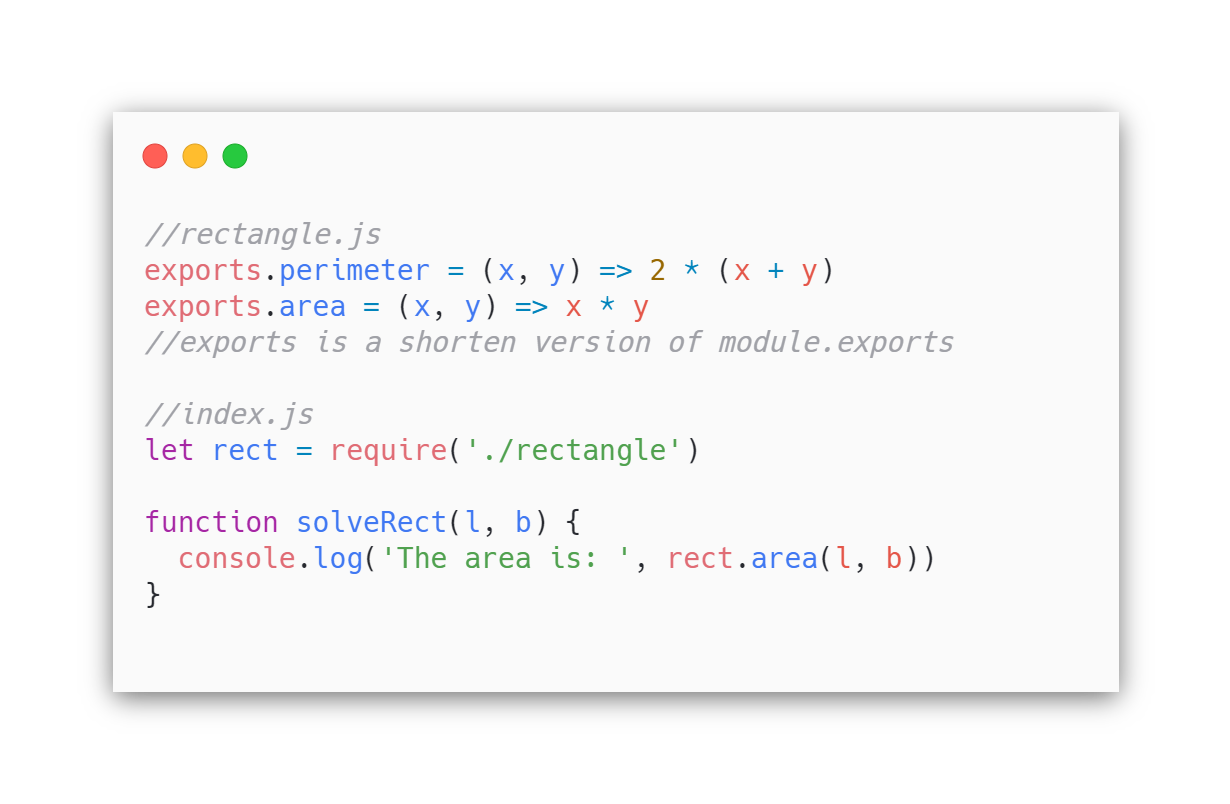
\includegraphics[width=\textwidth]{assets/modulenode.png}
    \caption{Example of a module and how to import}
    \label{fig:node-module}
\end{figure}

The module variable gives access to the current module definition in a file that can be exported using \textit{module.exports} or his shortand \textit{exports}.
The \textit{require} function is used to import a module.
There are several categories of module:
\begin{itemize}
    \item file-based modules
    \item core modules - part of Node's core like \textit{path}, \textit{fs}, or \textit{util}
    \item external modules - third-party modules installed using a package manager.
\end{itemize}


A module can be included using the \textit{require} function. A file-based module can be imported with \textit{require(module)} specifying the relative path to the file. It is enough for the core and external module to specify the module name, and Node will automatically look for external modules starting from \textit{node\_modules} folder up the hierarchy until the module is found.

\pagebreak

\subsubsection*{First-class functions and closures}
Node.js relies heavily on first-class functions and closures. A first-class function is a function that can be treated the same way as any other variable. For example, that can be passed as an argument to another function.
A closure is a function defined inside another function that has access to all the variables declared in the outer function (outer scope).
The inner function will continue to have access to the other variables from the outer scope even after the external function has returned.

\subsubsection*{Callback and Error handling}
Node.js is single-threaded, but at the same time, it can achieve a fast rate of completion of work. It is possible because of the judicious use of callbacks, the asynchronous execution of I/O requests, like file accesses or long-running processing that can be done independently behind the scenes.

Node.js continuously executes an event loop consisting of several phases:
\begin{itemize}
    \item timers - executes callbacks scheduled by \textit{setTimeout()} and \textit{setInterval}
    \item I/O callbacks - executes almost all calbacks with the exception od close callbacks and timers
    \item idle, prepare - internally used
    \item poll - retrieve I/O events, incoming connections, data, and others.
    \item check - \textit{setImmediate()} callbacks
    \item close callbacks - close callbacks like \textit{socket.on('close', ...)}
\end{itemize}
Each of these phases maintains its own separate queue, and the Node.js event loop picks up requests from each of these queues, and handles them. 

\subsection*{Networking}
Since network operations can cause unexpected delays and data is not instantaneously available, there is a need to write applications recognizing the asynchronous nature of communication. Network communications happens using the HTTP Client-Server communication protocol using the http module. Using this module is possible to create a server with \textit{http.createServer((res,req) +> {...})} and make it listen with \textit{server.listen(port,...)}.
The incoming messages are available through the \textit{req} parameter.

\subsection*{Express}
Express is the most popular third-party framework for building web servers. It is a fast, unopinionated, minimalist web framework for Node.js. It provides a robust set of features, and there are many third-party middlewares to extend functionality. An express application can be easily created using \textit{express-generator} through NPM.

A middleware provide a lot of plug-in functionality that can be used within your Express application. For example, \textit{morgan} is a plugin that can be used for logging

\subsubsection*{Router}
Express support routing URI through \textit{app.all, app.get, app.post, app.put} and \textit{app.delete} methods. This methods can be used to construct REST service:

\begin{center}
    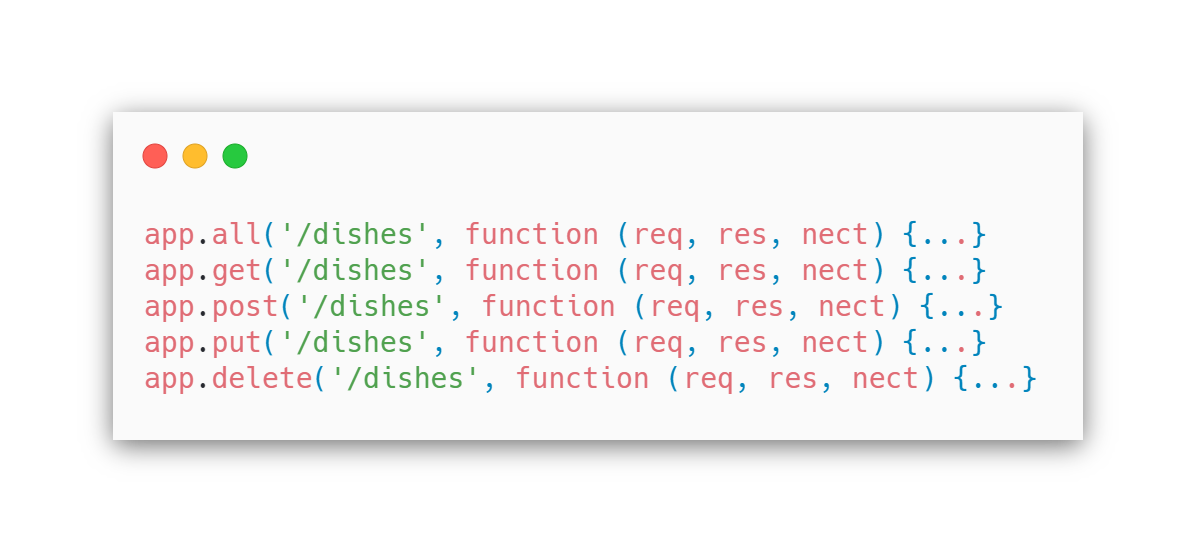
\includegraphics[width=0.8\textwidth]{assets/router.png}
\end{center}

It is possible to specify URI with parameters and to parse the body of a request using the \textit{body-parser} module.

There is also \textit{Express Router} for creaing mini-express application with routing abilities using \textit{myRouter = express.Router()} and then \textit{myRouter.route('/');}.

\subsection*{Authentication}
In Express, a request/response can pass through several middlewares that elaborate and propagate the modified request/response to the following middleware. For example, middleware could control if a request contains the necessary information to authenticate the user. If the user can be authenticated, the request can be propagated using the next() function; otherwise, it returns an error. 

\subsubsection*{Passport}
A node module that is an authentication middleware for Node.js. It is modular and flexible, it supports various strategies for authentication (local, openID, Oauth singgle sign-on, ...) and sessions.
Passport can be combined with Mongoose to simplify building login with username and password. It makes available Mongoose schema support for managing users, and it adds username, hash, and salt fields to store the username, the hashed password, and the salt value. It also provides additional methods to the User schema to support local authentication

\begin{center}
    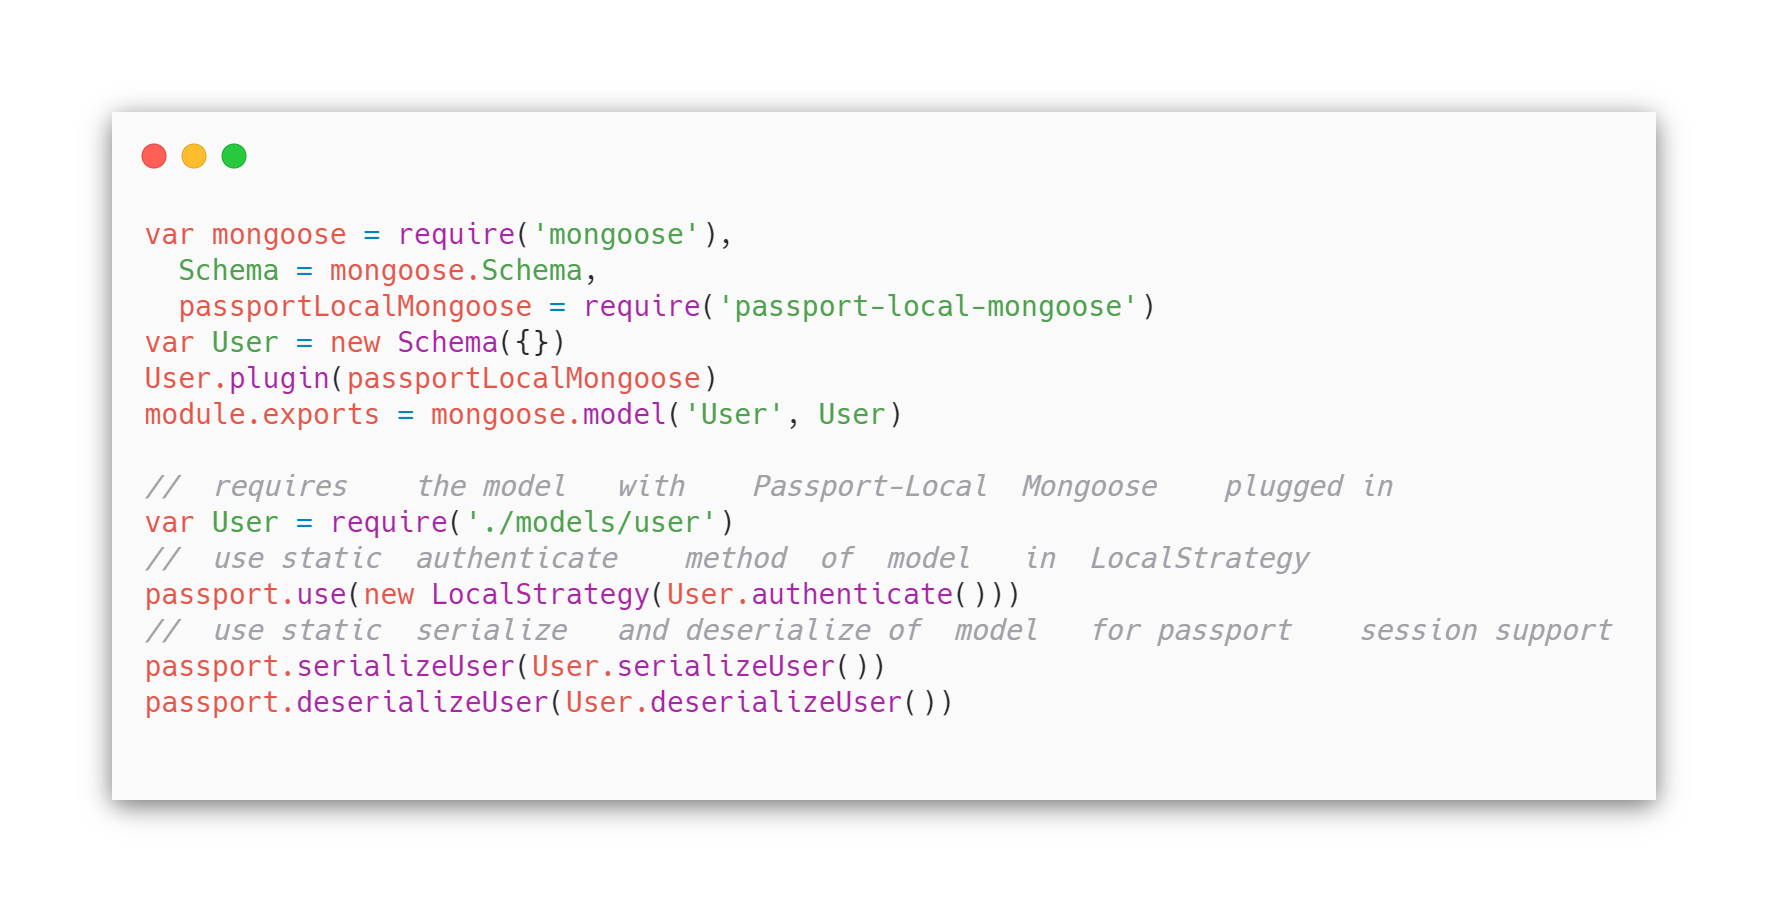
\includegraphics[width=0.8\textwidth]{assets/passport-mongoose.png}
    \label{fig:passport-mongoose}
\end{center}

Is it also possible to implement token-based authentication, especially if the server must be stateless and scalable or if the authentication should be shared between multiple servers. Token-based authentication helps to handle Cross-Origin resource sharing (CORS) problems and Cross-site request forgery.
The workflow is:
\begin{enumerate}
    \item User requests access with username and password
    \item Server validates credentials
    \item Server create a signed token and send it to the client (nothing is stored in the server)
    \item All subsequent requests from the client should include the token
    \item Server verifies the token and responds with data if validated
\end{enumerate}

To achieve token-based authentication in Express is possible to use jsonwebtoken and Passport-JWT modules. Passport-JWT creates and configures a new Passport strategy based on JWT authentication. It is possible to extract the JWT from an incoming request.

\subsubsection*{Sessions}
Sessions uses a combination of cookies and server-side storage to track users. A session is stored by default in a permanent memory server-side and it can be wiped out when the server restarts. It can be implemented using a middleware.

\begin{center}
    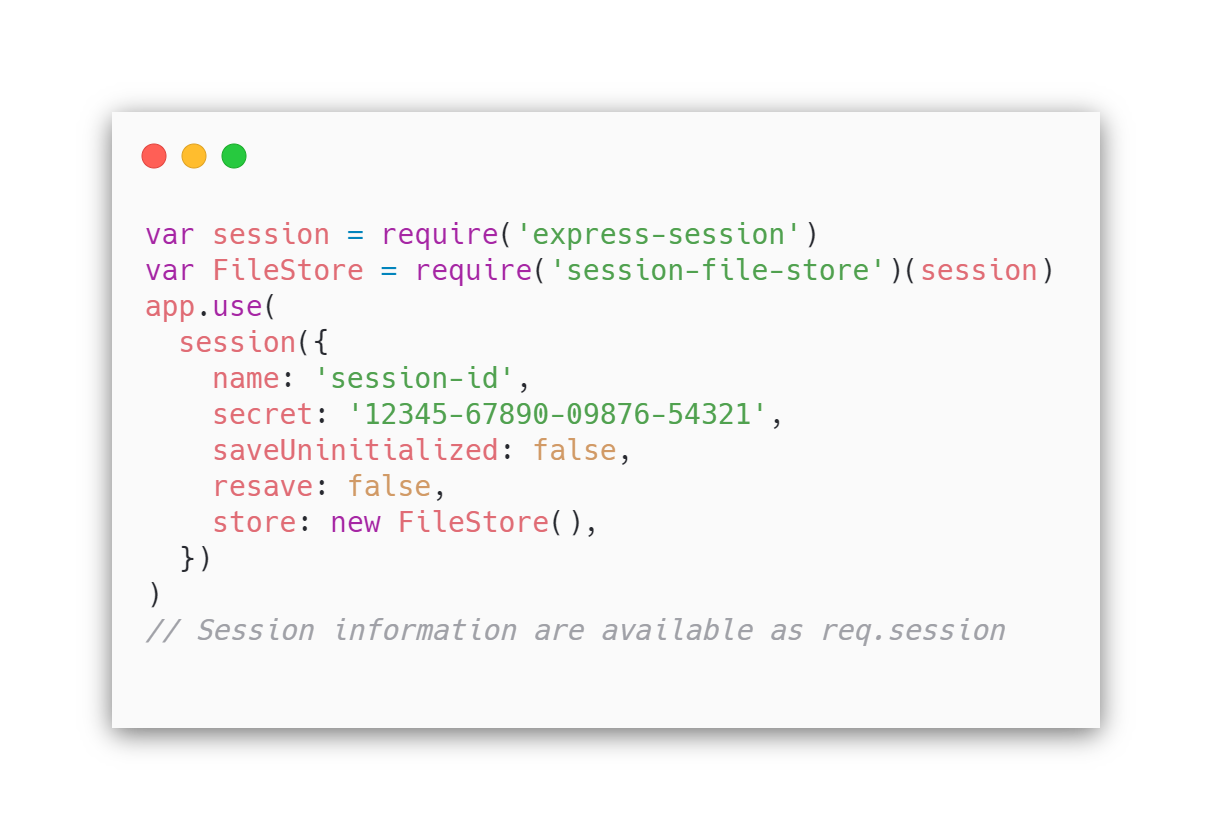
\includegraphics[width=0.8\textwidth]{assets/session.png}
    \label{fig:session}
\end{center}


\section*{MongoDB}

MongoDB is a document-based NoSQL DB. The document is a self-contained piece of information; it is possible to have a collection of documents, while a DB is a set of collections. A collection is a set of documents; a document is effectively a JSON file with some additional features. 
A NoSQL server can support multiple DBs. 
NoSQL's best features are scalability, availability, consistency, partition tolerance, and ease of deployment.

In MongoDB, documents are stored in a BSON (Binary JSON) format. It supports length prefix on each value, information about the field value type, and additional primitives type not supported by raw JSON like UTC date-time, raw binary, and ObjectID.

An ObjectID is a mandatory field \textit{\_id} created by MongoDB when a document is inserted.
MongoDB driver provides a high-level API for a Node application to interact with the MongoDB server for performing operations like connection, insertions, deletions, updates, and documents querying.

\subsection*{Mongoose ODM}
Mongoose ODM is a node module that gives a specific structure to documents and enforces the structure among all the applications. MongoDB stores data in the form of documents, but no structure is imposed on the document. Any document can be stored in any collection and relies on the developer's discipline to maintain the structure of the documents. MongoDB stores data in the form of documents, but no structure is imposed on the document. Any document can be stored in any collection and relies on the developer's discipline to maintain the structure of the documents.

\subsubsection*{Mongoose Schema}
It defines all the fields of the document and their types. It can do validation. Various schema types are String, number, date, buffer, boolean, mixed, ObjectID, and array. The schema is used to create a model function. Mongoose's schema types include String, Number, Date, Buffer, Boolean, Mixed, ObjectID, and Array. The Array schema type allows the creation of an array of sub-documents inside the document. Once a schema is defined, it is used in Mongoose to create a model function, which allows determining the structure for the documents in the database. Schemas can be nested to enable supporting embedded or sub-documents. 

\subsubsection*{Mongoose Population}
NoSQL databases like MongoDB usually do not explicitly support relations like the SQL databases. All documents are generally expected to be self-contained.
However, it is possible to store references to other documents within a document by using ObjectIds.

\begin{center}
    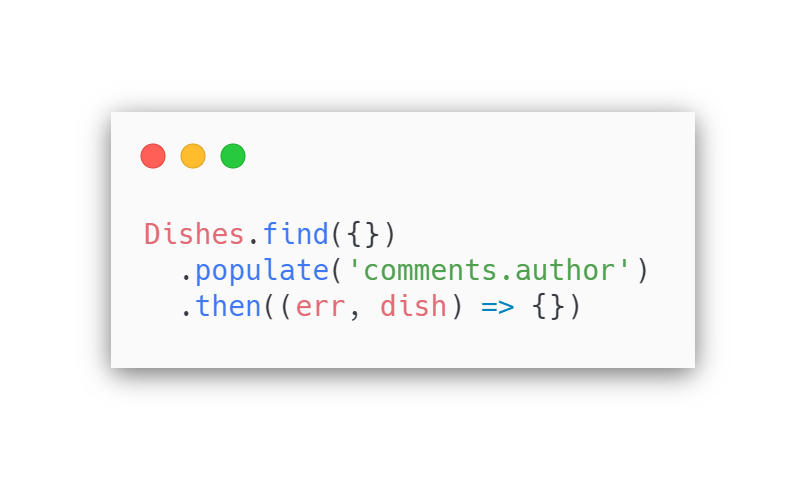
\includegraphics[width=0.8\textwidth]{assets/population.png}
\end{center}

Population automatically replaces specified paths within a document with documents from another collection using cross-reference with ObjectIds helps.
For example, an object 'comment' can have a rating, a comment, and an author.  It is possible to populate a Dish with a list of comments using Mongoose Population.